% don't remove the folling lines, and edit the defintion of \main if needed
\documentclass[../report.tex]{subfiles}
\providecommand{\main}{..}
\IfEq{\jobname}{\currfilebase}{\AtEndDocument{\biblio}}{}
% until here

%\newcommand{\mlna}{\langle \ln\!A \rangle}
%\newcommand{\nmu}{N_\mu}
%\newcommand{\lnnmu}{\ln\!\nmu}
%\newcommand{\xmax}{X_\text{max}}
%\newcommand{\nmult}{N_\text{mult}}
%\newcommand{\tocite}{{\bf REF}}
%\newcommand{\si}[1]{\ensuremath{\text{#1}}}
%\newcommand{\SI}[2]{\ensuremath{#1\,\si{#2}}}

%\newcommand{\pt}{p_\mathrm{T}}

\begin{document}

\section{Future physics opportunities with ions and proton beams at the LHC}
%%%%%%%%%%%%%%%%%%%%%%%%%%%%%%%%%%%%%%%%%%%%%%%%%%%%%%%%%%%%%%%%%%%%%%
\textbf{Coordinators}:  Iwona Grabowska-Bold (AGH UST, Krak\'ow)
\linebreak
\textbf{Contributors}: Mateusz Dyndal (DESY), Iwona Grabowska-Bold (AGH UST, Krak\'ow), Samira Hassani (Universit\'e Paris-Saclay), Mariola Klusek-Gawenda (NIP PAS, Krak\'ow), Laurent Schoeffel (Universit\'e Paris-Saclay ), Peter Steinberg (BNL)

{\footnotesize Acknowledgments:\\
Research of IGB was supported in part by Polish National Science Centre grant DEC-2016/23/B/ST2/01409,
by the AGH UST statutory tasks No. 11.11.220.01/4 within subsidy of the Ministry of Science and Higher
Education, and by PL-Grid Infrastructure.\\
The work of M.KG was supported by the Polish National Science Center Grant No. DEC-2014/15/B/ST2/02528.
}

%%%%%%%%%%%%%%%%%%%%%%%%%%%%%%%%%%%%%%%%%%%%%%%%%%%%
\subsection{Physics of $\gamma \gamma$ interactions in heavy-ion collisions}
\label{sec:upc}
%%%%%%%%%%%%%%%%%%%%%%%%%%%%%%%%%%%%%%%%%%%%%%%%%%%%%%%%%%%%%%%%%%%%%%

Heavy-ion beams are composed of nuclei which carry electric charge $Ze$~($e$ is the electron charge and $Z$ is the atomic number). Moreover, they are accelerated to nearly the speed of light, thus they generate extremely large electromagnetic~(EM) fields. These EM fields can also interact either with another nucleus or with its EM fields.
Therefore, besides nuclear hadronic interactions, EM
interactions also occur in ultra-relativistic heavy-ion collisions.
These EM interactions can be studied in so-called ultra-peripheral
collisions~(UPC) which occur when the distance between two nuclei in the transverse plane is larger than two times the nuclear radius, and hadronic interactions are thus suppressed~\cite{Bertulani:2005ru}.

A broad range of processes can be studied with $\gamma\gamma$ interactions in UPC. In the following, a few examples of photon-induced processes are considered at the HL-LHC: exclusive production of $\mu^+\mu^-$ or $p\bar{p}$ pairs, a rare process of light-by-light~(LbyL) scattering and a potential of searches for axion-like particles~(ALP).

%-------------------------------------------------------------------
\begin{figure}[!hbt]
\centering
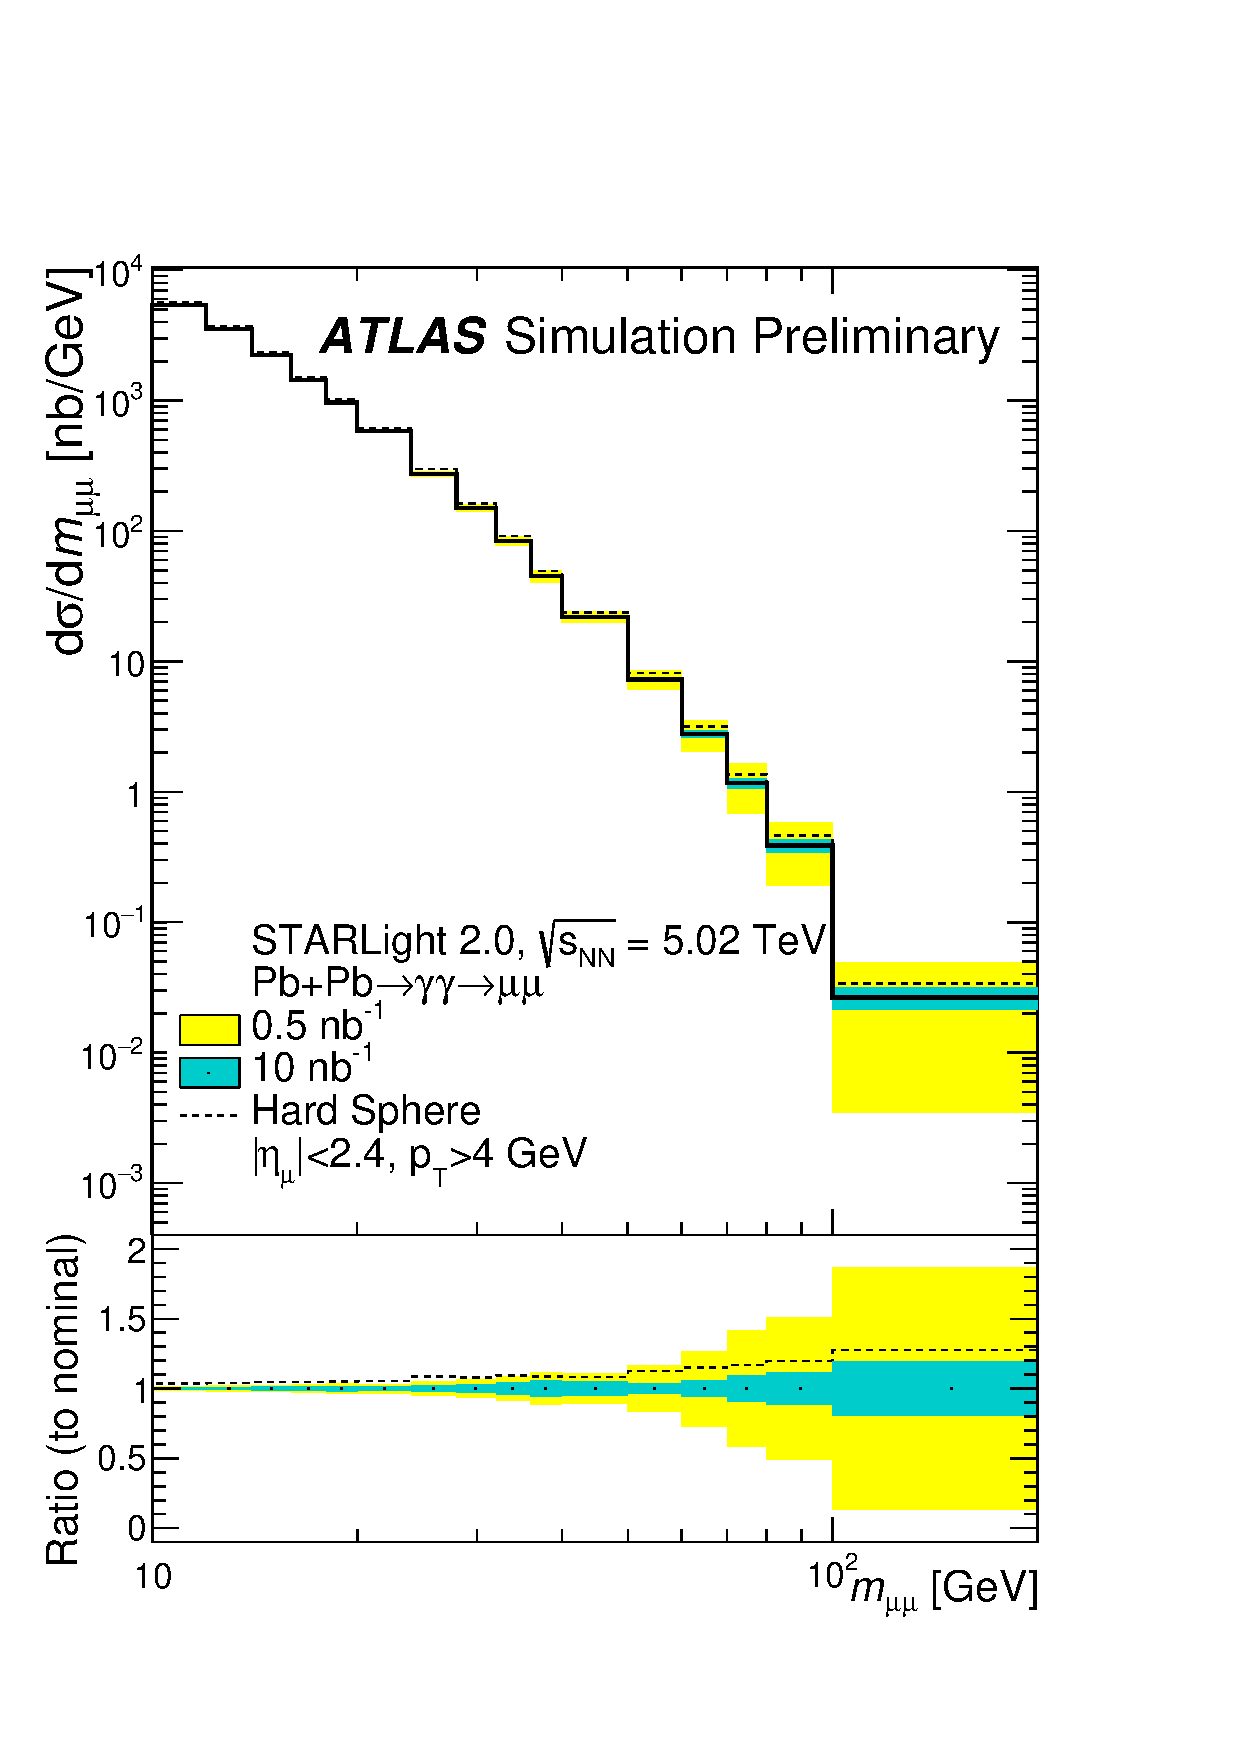
\includegraphics[width=0.50\linewidth]{\main/beyond/fig/fig_01.pdf}
\caption{
(Upper)~Differential cross section for exclusive production of the di-muon pairs as a function of the di-muon mass for
$10<m_{\mathrm{\mu\mu}}<200$~GeV extracted from STARLight. Two
scenarios are considered for the nuclear geometry: a realistic skin
depth of the nucleus~(solid line) or a hard sphere~(dashed
line). (Bottom)~Ratio to nominal as a function of the di-muon mass,
where "nominal'' stands for the realistic skin depth of the nucleus.
 Shaded bands represent expected statistical uncertainties for integrated luminosity of $0.5~\mathrm{nb}^{-1}$~(yellow), and $10~\mathrm{nb}^{-1}$~(cyan).}
\label{fig:mumu}
\end{figure}
%-------------------------------------------------------------------

Exclusive production of di-muon pairs~($\gamma\gamma\rightarrow \mu^+\mu^-$) in UPC can offer a precision-like measurement of photon fluxes associated with ion beams, and as such can be used to constrain predictions for the other processes covered in this section. The cross section at high pair mass is also sensitive to the nuclear geometry assumed in the calculations. Figure~\ref{fig:mumu} presents a differential cross section as a function of the invariant mass of the di-muon system in the range of 10-200~GeV with expected statistical uncertainties represented by two bands corresponding to integrated luminosities of $0.5~\mathrm{nb}^{-1}$ and
$10~\mathrm{nb}^{-1}$. Two scenarios are considered for the nuclear
geometry: a realistic skin depth of the nucleus or a hard sphere~\cite{Barrett:1977}.
For the $10~\mathrm{nb}^{-1}$ scenario, a significant reduction of the
statistical uncertainty is expected for the highest $m_\mathrm{\mu\mu}$ bin which spans 100-200~GeV.  This will help in reducing uncertainties from the modeling of the nuclear charge distributions.
The expected upgrades of the ATLAS Zero Degree Calorimeters~(ZDC) in the LHC Run 3 will also be important for isolating the contributions from dissociation.

Exclusive production of $p\bar{p}$ pairs~($\gamma\gamma\rightarrow p\bar{p}$) in heavy-ion collisions is considered as a process which can help verify the existing theoretical approaches. It has been demonstrated that the existing $\gamma\gamma\rightarrow p\bar{p}$ experimental data~\cite{Kuo:2005nr} from the Belle Collaboration can be successfully described by implementation of several components~\cite{Klusek-Gawenda:2017lgt}: the non-resonant proton exchange, $s$-channel tensor meson exchange and the hand-bag model~\cite{Diehl:2002yh}. Figure~\ref{fig:ppbar} shows distributions of invariant mass of the $p\bar{p}$ system, $W_{\gamma\gamma} = M_{p\bar{p}}$~(left panel) and of the difference
of rapidities for protons and anti-protons, $y_{\mathrm{diff}} = y_\mathrm{p} - y_{\mathrm{\bar{p}}}$~(right panel).
The ALICE Collaboration can measure $p\bar{p}$ pairs in Pb+Pb collisions at mid-rapidity~($|y|$ < 0.9). The ATLAS and CMS experiments will improve the acceptance in rapidity in Run~4 to cover $|y|$ < 4.0.
The LHCb Collaboration could also provide a complementary measurement of $p\bar{p}$ production in the forward region~(2 <$\eta$ < 4.5).  Corresponding kinematic requirements on transverse momenta and rapidity or pseudorapidity specific for each experiment are presented in the figure legend. The calculations are made for Pb+Pb collisions with $\sqrt{s_{\mathrm{NN}}}$ = 5.52~TeV.
The total cross section predicted for the CMS acceptance is $\sigma$ = 793~$\mu$b, while ATLAS, LHCb and ALICE requirements lead to $\sigma$ = 248, 125 and 105~$\mu$b, respectively.

%-------------------------------------------------------------------
\begin{figure}[!h]
        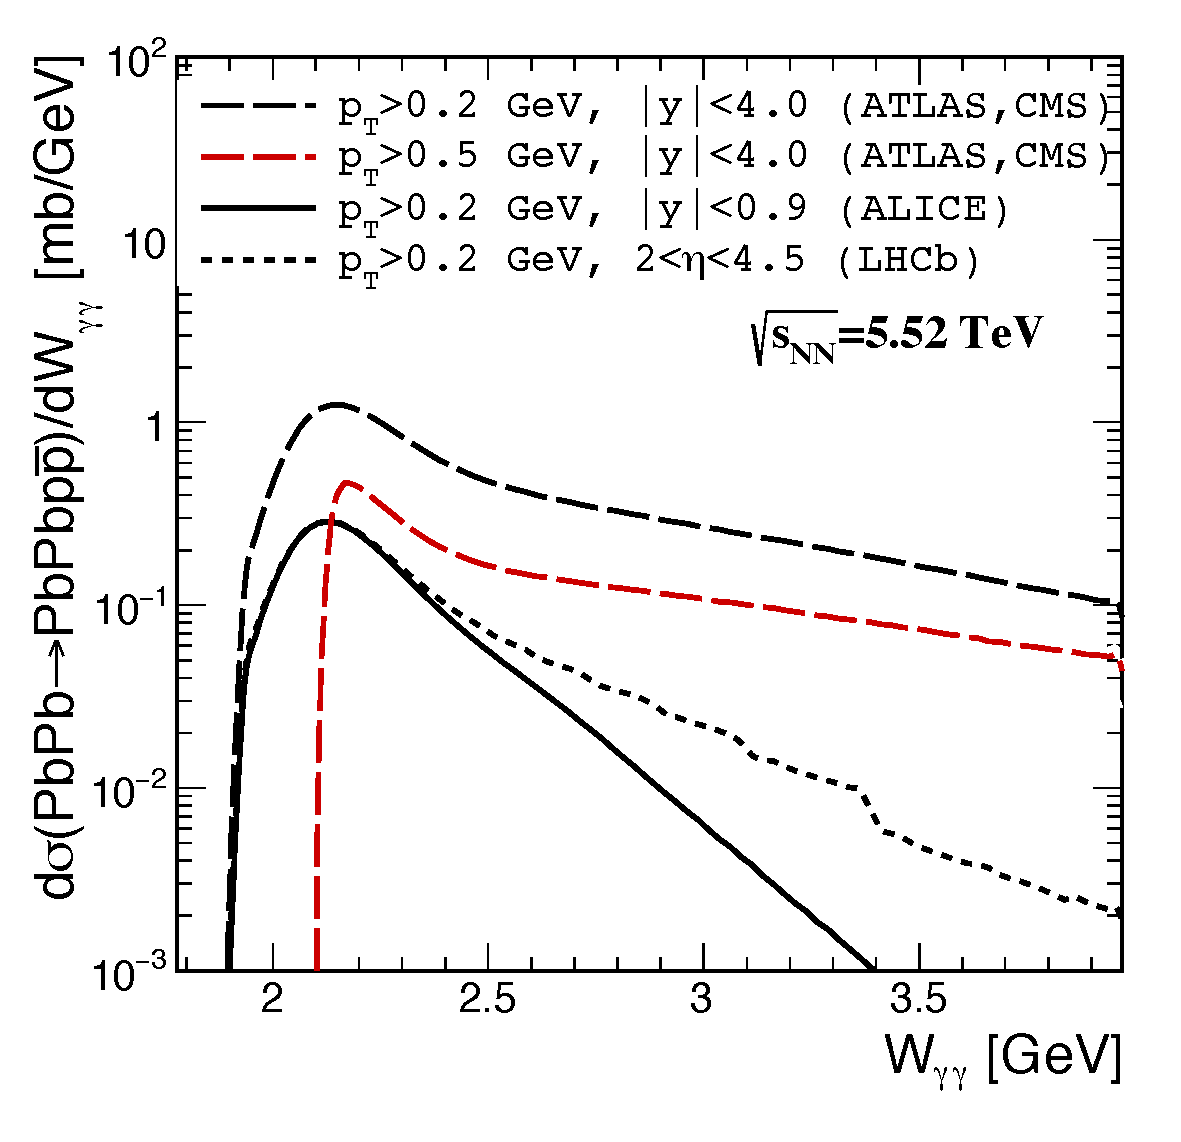
\includegraphics[scale=0.375]{\main/beyond/fig/dsig_dw_4exp_plus_y4_nucl_5520GeV.pdf}
        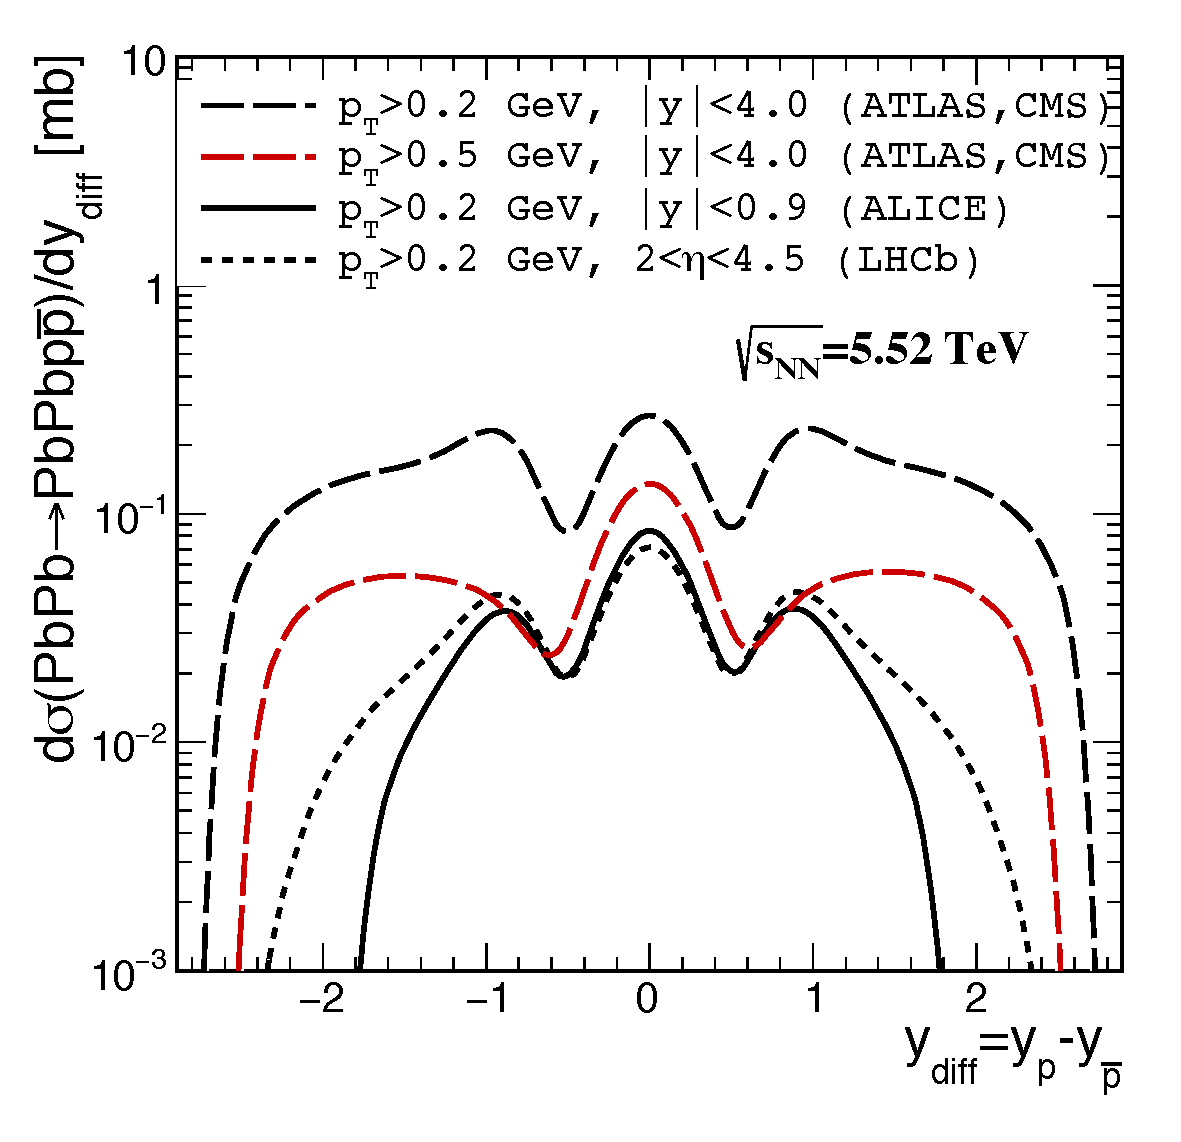
\includegraphics[scale=0.375]{\main/beyond/fig/dsig_dydiff_4exp_plus_y4_nucl_5520GeV.pdf}
        \caption{
                Differential cross section as a function of $p\bar{p}$
                invariant mass~(left) and rapidity
                distance between proton and anti-proton~(right)
                in Pb+Pb collisions at $\sqrt{s_{\mathrm{NN}}}$=5.52\,TeV
                for four experimental acceptance requirements.
        }
        \label{fig:ppbar}
\end{figure}
%-------------------------------------------------------------------


From the left panel of Figure~\ref{fig:ppbar} one can deduce that the dependence on invariant mass of the $p\bar{p}$ pair is sensitive to the rapidity/pseudorapidity requirement. The cut-off at the minimal value of $W_{\gamma\gamma}$ is determined by the minimum $\pt$ requirement.
The $y_{\mathrm{diff}}$ distribution shown on the right panel of Figure~\ref{fig:ppbar} seems to be particularly interesting. 
The broad maximum at $y_{\mathrm{diff}}=0$ corresponds to the region with $|\cos \theta|$ < 0.6, where $\theta$ denotes the angle of the outgoing nucleon relative to the beam direction in the center-of-mass frame. An observation of further peaks could be a good test to constraint the theoretical models. The experimental requirements
imposed on $\pt$ do not distort the maxima. If the structures present in the $y_{\mathrm{diff}}$ distribution can be confirmed experimentally, the study of production of $p\bar{p}$ pairs
in UPC can provide new information compared to the currently available data for $\gamma\gamma\rightarrow J/\psi \rightarrow e^+e^-$ production~\cite{Kryshen:2017jfz,Abbas:2013oua}.


An evidence of the rare process of LbyL scattering has been established by ATLAS and CMS Collaborations in 2015 Pb+Pb collisions~\cite{Aaboud:2017bwk,Sirunyan:2018fhl} with an integrated luminosity of about $0.4\;\mathrm{nb}^{-1}$. That process can be studied with higher precision using heavy-ion data collected at the HL-LHC. The left panel of Figure~\ref{fig:lbyl} presents a differential cross section as a function of the di-photon rapidity for LbyL scattering for photons with $|\eta^\gamma|<4$ with two photon $\pt^\gamma$ thresholds: 2.5 and 2.0~GeV. The LbyL scattering occurs in the central region: 91\% of the integrated cross section is within $|\eta^\gamma|<2.37$. A strong dependence on the $\pt^\gamma$ is however observed. The cross section increases by a factor of two when the single photon $\pt^\gamma$ threshold is lowered by half a GeV from 2.5 to 2.0~GeV. The corresponding integrated cross sections in the fiducial region are 112~nb for $\pt^\gamma>2.5$~GeV and 221~nb for $\pt^\gamma>2.0$~GeV. However, triggering on photons with $\pt^\gamma<2.5$~GeV might be challenging, and therefore a dedicated trigger strategy needs to be developed for LbyL event candidates.

The right panel of Figure~\ref{fig:lbyl} shows a detector-level  acoplanarity~(=$|1-(\phi^\gamma_1-\phi^\gamma_2)/\pi|$) distribution for the di-photon system from LbyL signal and two background processes originating from exclusive production of di-electron pairs~($\gamma\gamma\rightarrow\,e^+e^-$) and di-photons produced in central exclusive production~($gg\rightarrow \gamma\gamma$). 
About 640 LbyL events pass the selection requirements for acoplanarity below 0.01 and 
$\pt^\gamma>2.5$~GeV in 5.02~TeV \PbPb~collisions with an integrated luminosity of 10\,nb$^{-1}$, 
in comparison to about 13 events observed in the 2015 data set. 
The signal events are peaked at acoplanarities close to zero, while the background processes are distributed either uniformly (di-photons from central exclusive production) or even grow with acoplanarity ($e^+e^-$ pairs from exclusive di-electron production). 

%-------------------------------------------------------------------
\begin{figure}[!hbt]
\centering
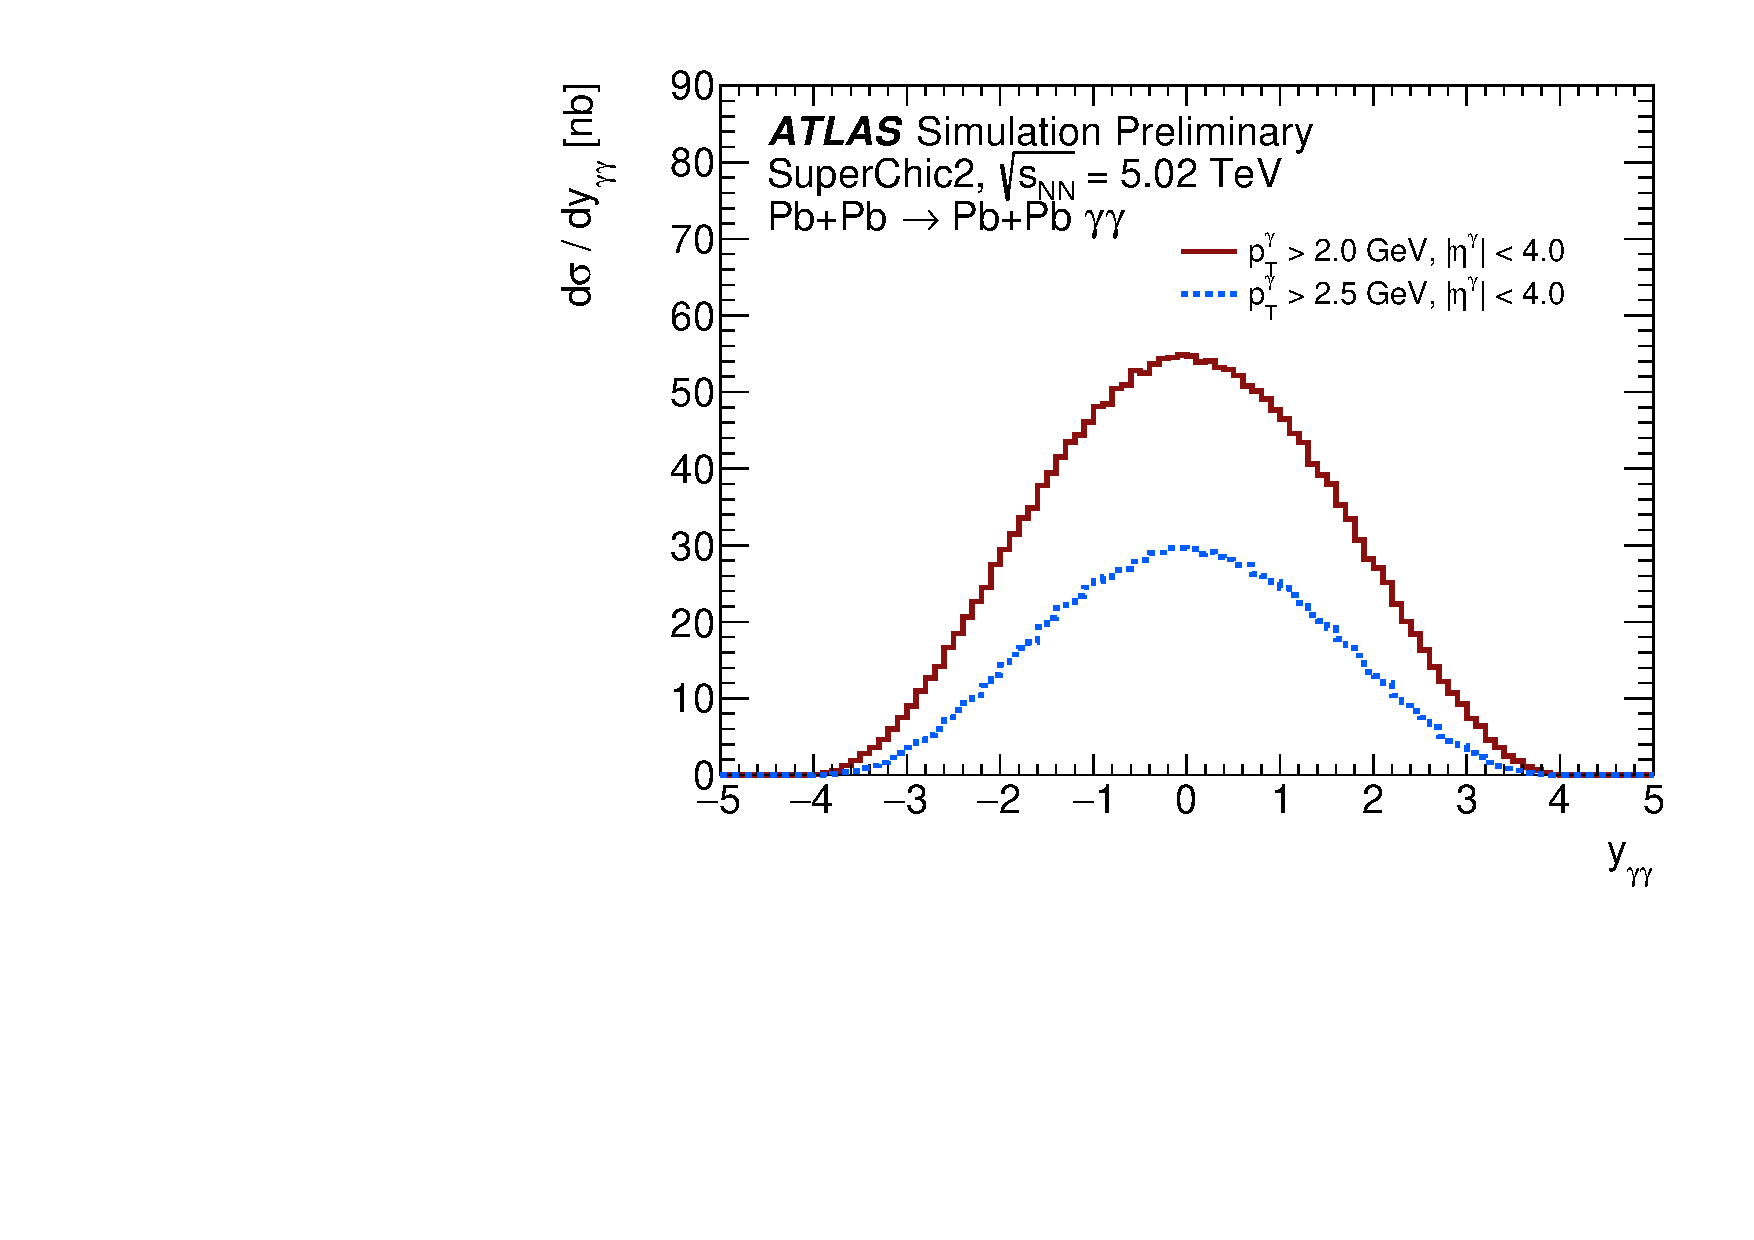
\includegraphics[width=0.49\linewidth]{\main/beyond/fig/fig_02.pdf}
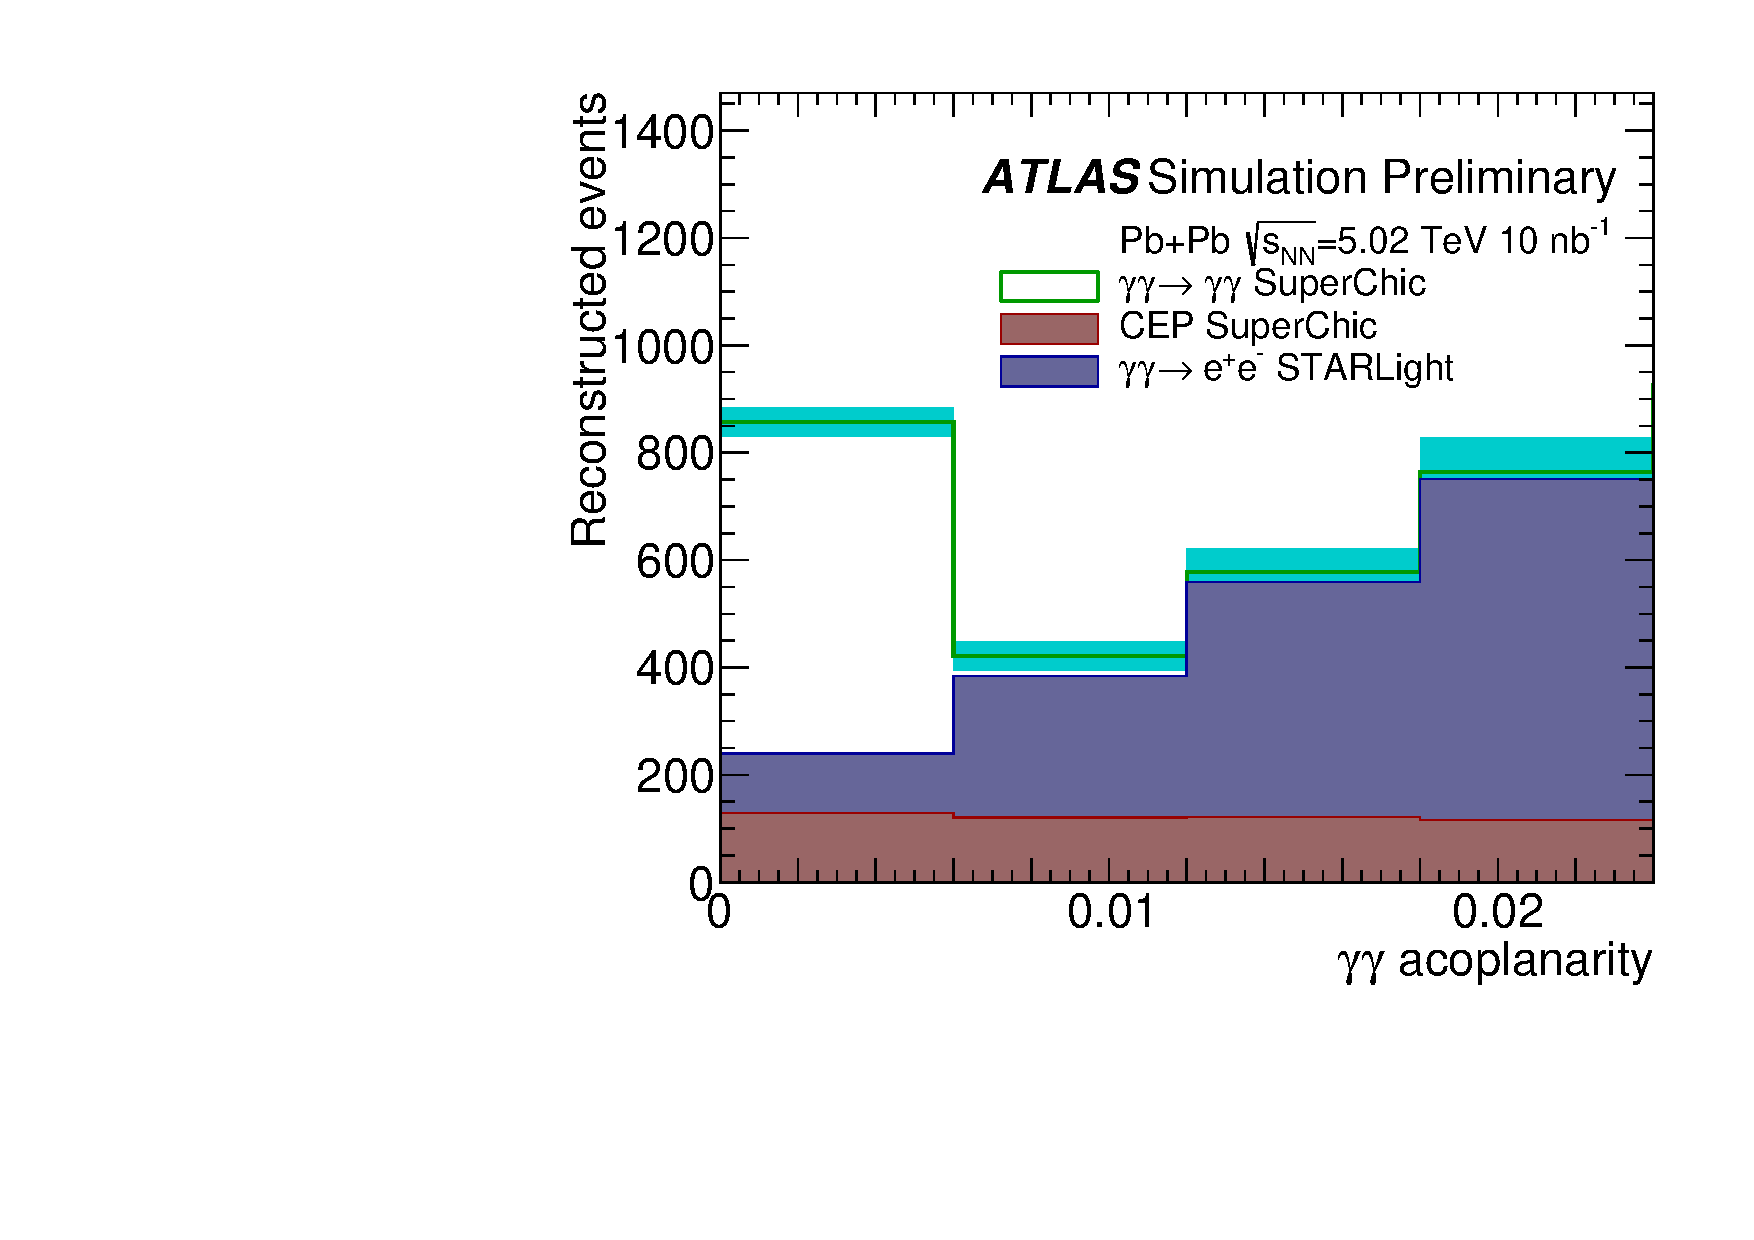
\includegraphics[width=0.425\linewidth]{\main/beyond/fig/fig_03a.pdf}
\caption{
(Left)~Predicted differential cross section as a function of the di-photon rapidity for LbyL scattering for photons with
$\pt^\gamma>2.5$~GeV~(dashed) or $\pt^\gamma>2.0$~GeV~(solid), and
$|\eta^\gamma|<4$ extracted from SuperChic2.
(Right) Detector-level acoplanarity distribution of the di-photon system for photons from the LbyL signal and background processes in
  5.02~TeV Pb+Pb collisions with an integrated luminosity of
  $10~\mathrm{nb}^{-1}$. The shaded band in cyan represents expected statistical uncertainties.
}
\label{fig:lbyl}
\end{figure}
%-------------------------------------------------------------------

The LbyL process can also be studied at lower di-photon masses. The differential cross sections as a function of the di-photon mass can be evaluated taking into account acceptance of the ALICE experiment, i.e. pseudorapidity limited to $|\eta^\gamma|<0.9$ and relatively low energies of outgoing photons. At lower energies~($W_{\gamma\gamma} <$ 4~GeV) meson resonances~\cite{Klusek-Gawenda:2018ijg} may play an important role in addition to the Standard Model box diagrams~\cite{dEnterria:2013zqi,Klusek-Gawenda:2016euz}
or double photon fluctuations into light vector mesons~\cite{Klusek-Gawenda:2016euz} or two-gluon exchanges~\cite{Klusek-Gawenda:2016nuo}.
%-------------------------------------------------------------------
\begin{figure}[!h]
        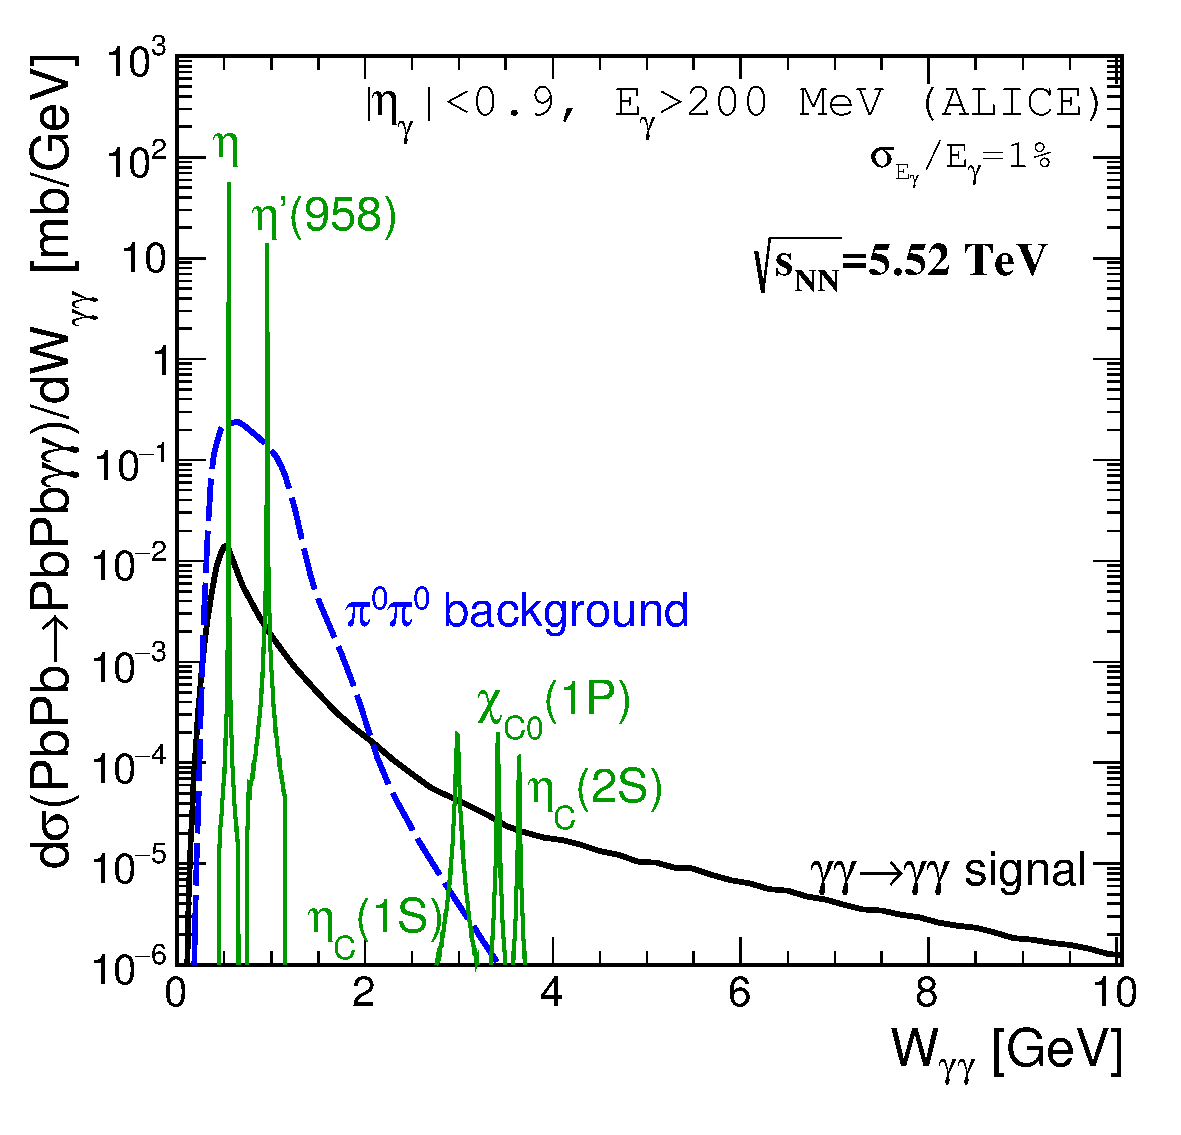
\includegraphics[scale=0.375]{\main/beyond/fig/dsig_dW_pi0pi0_mesons_ALICE_from_gaussian_energy_resolution.pdf}
        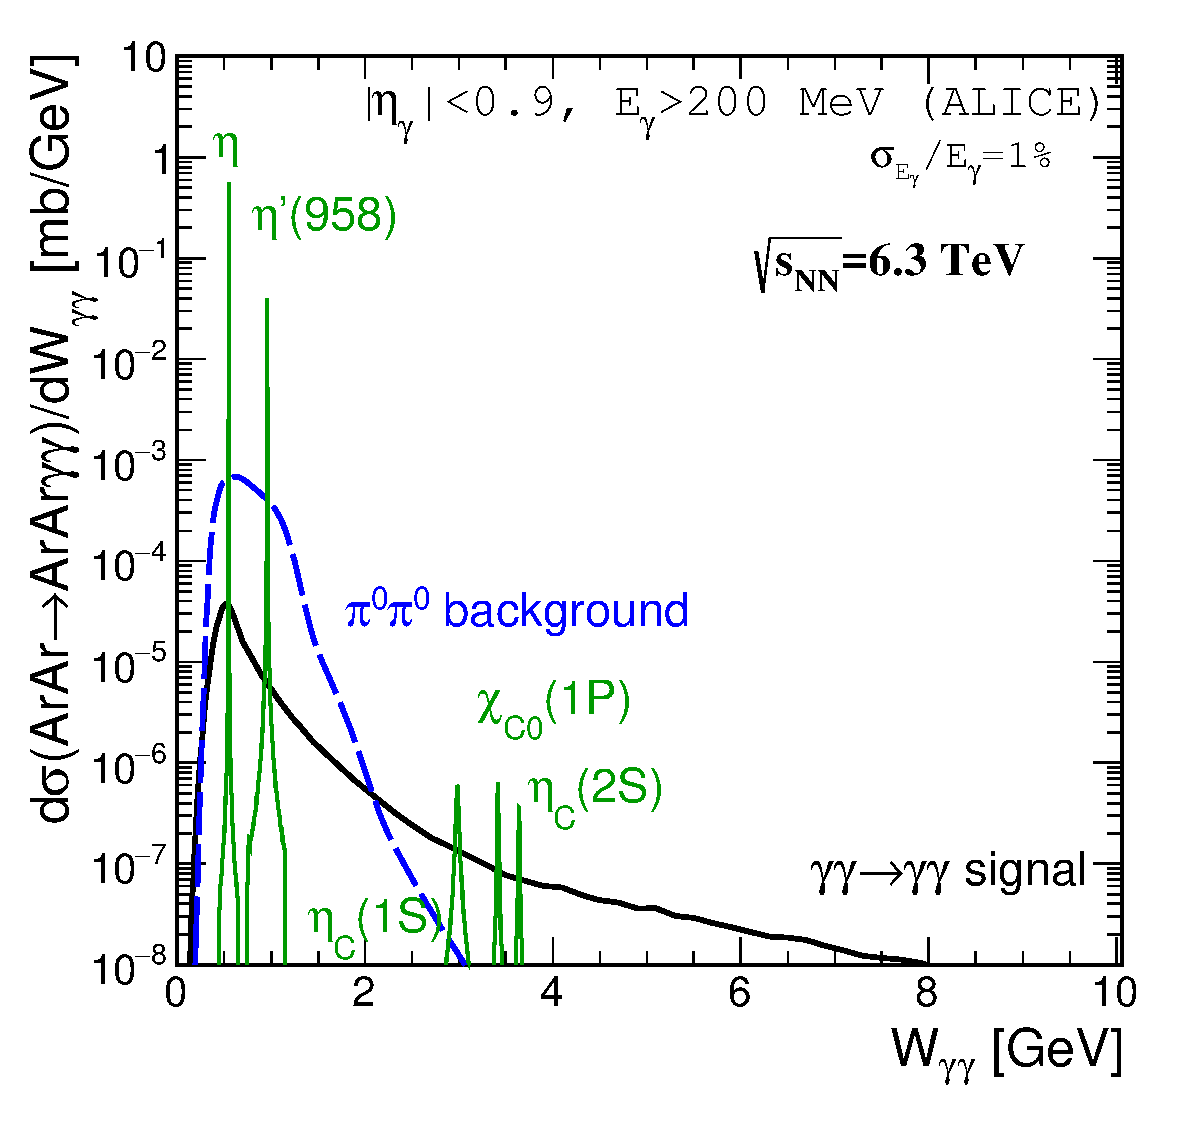
\includegraphics[scale=0.375]{\main/beyond/fig/dsig_dW_pi0pi0_mesons_ALICE_from_gaussian_energy_resolution_ArAr.pdf}
        \caption{
                Di-photon invariant mass distribution for mid-rapidity for Pb+Pb collisions at $\sqrt{s_{\mathrm{NN}}}$=5.52\,TeV~(left) and Ar+Ar collisions at $\sqrt{s_{\mathrm{NN}}}$=6.3\,TeV~(right).
        }
        \label{fig:lbyl_alice}
\end{figure}
%-------------------------------------------------------------------
Figure~\ref{fig:lbyl_alice} shows predictions dedicated for the ALICE detector with photon acceptance in $|\eta_{\gamma}|$ < 0.9, and photon energy $E_{\gamma}$ > 200~MeV for two systems: Pb+Pb collisions at 5.52~TeV~(left panel) and Ar+Ar collisions at 6.3~TeV~(right panel). Presented results include the effect of the experimental energy resolution~\cite{Acharya:2018yhg}.
The black-solid lines depict LO QED fermionic box mechanism.
In the numerical calculations, the inclusion of leptons and quarks is sufficient. Presented results for the $\gamma\gamma\to\gamma\gamma$ process have been compared to other calculations from Refs.~\cite{Jikia:1993tc,Bern:2001dg,Bardin:2009gq}. A good agreement is found. The green-solid lines show nuclear results for the $s$-channel $\gamma\gamma\to$pseudoscalar/scalar/tensor resonances that contribute to the LbyL process.
In the present analysis, $\eta$, $\eta'(958)$, $\eta_c(1S)$, $\eta_c(2S)$, $\chi_{c0}(1P)$ mesons are considered.
Their masses, total widths and branching ratios are taken from PDG~\cite{Patrignani:2016xqp}.
The dominant background from the $\gamma\gamma\to\pi^0\pi^0$
process is depicted by the blue-dashed lines. It becomes non-negligible  only when one photon from each $\pi^0\to\gamma\gamma$ decay is reconstructed in the detector.
The experimental data for the $\gamma\gamma\to\pi\pi$ elementary cross section were very nice described in Ref.~\cite{Klusek-Gawenda:2013rtu}.
There simultaneously the total cross section and angular distributions for both charged and neutral pions are shown.
Following Ref.~\cite{Klusek-Gawenda:2013rtu}, here nine resonances,
$\gamma\gamma\to\rho^\pm\to\pi^0\pi^0$ continuum, Brodsky-Lepage and hand-bag mechanism are included. Figure~\ref{fig:lbyl_alice} shows that pionic background dominates at low invariant di-photon mass~(below 2~GeV).
In the same energy region, one can observe a very clear dominance of
$\eta$, $\eta'(958)$ mesons over boxes and background.
The inclusion of energy resolution has a significance mainly at
$\gamma\gamma\to\eta,\eta'\to\gamma\gamma$ resonance scattering.
This contribution is supposed to be measured with good precision.
%However, the resonance signal is modified including experimental energy resolution and a peak is about one order of magnitude smaller than without experimental resolution but the total cross section is of course still the same.
These results suggest that the ALICE Collaboration could measure LbyL scattering for $W_{\gamma\gamma}>$ 2~GeV in Pb+Pb collisions. The cross sections are about two orders of magnitude lower in the Ar+Ar system due to smaller electric charge associated with argon beams.


Axions and ALP are fundamental components of extensions of the Standard Model, occurring in most solutions of the strong CP problem~\cite{Peccei:1977hh,PhysRevLett.38.1440}. Recently an increasing interest has been paid to ALP masses
above 1~GeV~\cite{Bauer:2017ris}. In particular the Higgs discovery has set spin zero particles in the spotlight of searches for new physics, with scalar and pseudo-scalar particles (elementary or not) as heralds of new phenomena. An interesting feature is that ALP (generically labeled as $a$ in the following) in this mass range would induce an anomalous contribution to the LbyL, via the reaction:
$\gamma \gamma \rightarrow a \rightarrow \gamma \gamma$,
under the condition that the magnitudes of the EM fields associated
with the incident photon are large enough, typically $\left|\vec{E}\right| >10^{18}$~V/m.
This has triggered  the study presented in Ref.~\cite{Knapen:2016moh},
and then in Ref.~\cite{Knapen:2017ebd} using the recent observation of LbyL scattering published by the ATLAS experiment in Pb+Pb collisions~\cite{Aaboud:2017bwk}, where the electric field produced by the ultra-relativistic Pb is of the order of $10^{25}$~V/m (thus satisfying the above condition).

The potential of ALP searches in UPC Pb+Pb collisions is studied using detector-level quantities after the LbyL selection requirements are imposed. The overall selection efficiency (times acceptance) relative to generated events increases from about $40$\% to $65$\% for ALP masses ranging from $7$ to $80$~GeV. Also, the mass resolution varies from $0.5$~GeV at low masses (below $15$~GeV) up to $1$~GeV for larger masses. In the left panel of Figure~\ref{fig:alp} the expected mass distributions for three ALP signal mass values, and the main background from LbyL are shown. In this study, other sources of backgrounds are neglected, since they have been found to be small in the LbyL measurement~\cite{Aaboud:2017bwk}. The invariant mass distribution is used as the discriminating variable, with bin widths comparable to the expected resolution of a narrow resonant signal.
Upper limits are set on the product of the production cross section of
new resonances and their decay branching ratio into $\gamma
\gamma$. Exclusion intervals are derived using the CLs method~\cite{Read:2002hq} in the asymptotic approximation. The limit set on the signal strength $\mu$ is then translated into a limit on the signal cross section times branching ratio as presented in the right panel of Figure~\ref{fig:alp}.
%-------------------------------------------------------------------
\begin{figure}[!htbp]
\centering
  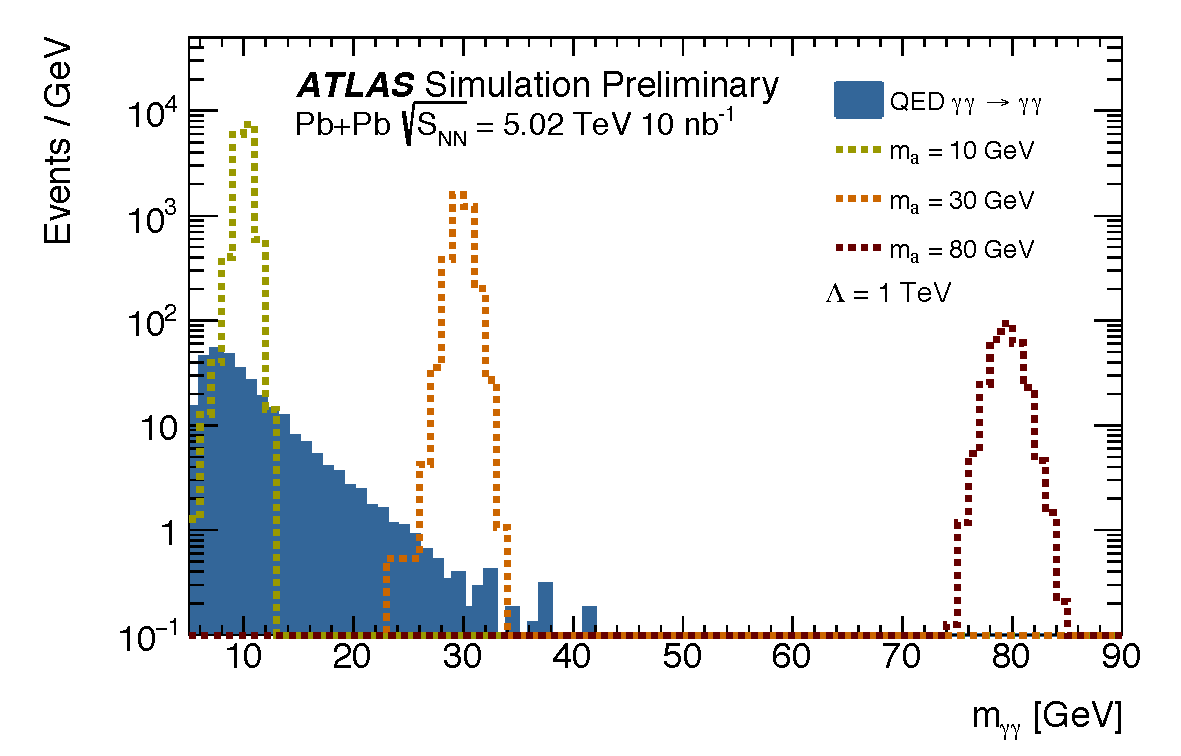
\includegraphics[scale=0.45]{\main/beyond/fig/fig_04.pdf}
  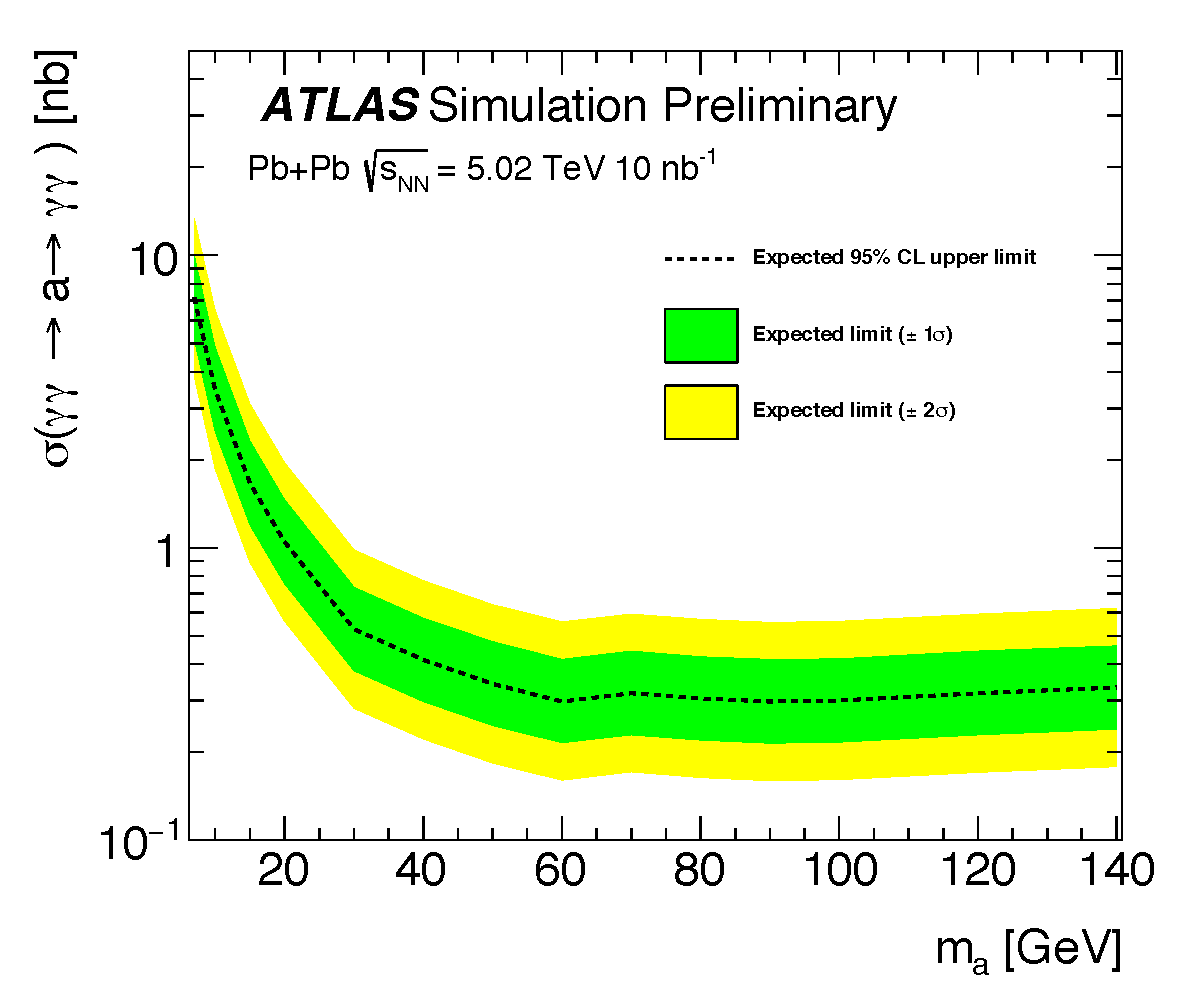
\includegraphics[scale=0.34]{\main/beyond/fig/fig_05a.pdf}
  \caption{(Left)~Mass distribution for the ALP signal
  shown for three values of the ALP mass: $m_\mathrm{a}=10, 30$ and
  $80$~GeV~(in red). Also shown (in blue) the LbyL background~(see
  text). All ALP mass points are generated with $\Lambda = 1$~TeV.
  (Right)~Expected $95$\% CLs upper limits on $\sigma_{a\rightarrow \gamma \gamma}$.}
  \label{fig:alp}
\end{figure}
%-------------------------------------------------------------------

In Figure~\ref{fig:alp-lambda-limits} two exclusion limits on the coupling along with the existing exclusion limits from the compilation presented in Ref.~\cite{Baldenegro:2018hng} are presented. The LHC 10~nb$^{-1}$ limit is derived using the analysis described above at $\sqrt{s_{\mathrm{NN}}}=5.02$~TeV. The LHC 20~nb$^{-1}$ limit is established using a combined analysis of the ATLAS and CMS data assuming similar acceptance and photon performance in the two experiments and nominal energy of $\sqrt{s_{\mathrm{NN}}}=5.52$~TeV.
Sensitivity of these analyses covers the range in ALP masses between $7$ and $140$~GeV, where the previous analysis~\cite{Knapen:2016moh} is also shown~(labeled as ATLAS 2016 in the figure).

%-------------------------------------------------------------------
\begin{figure}[!htbp]
\centering
  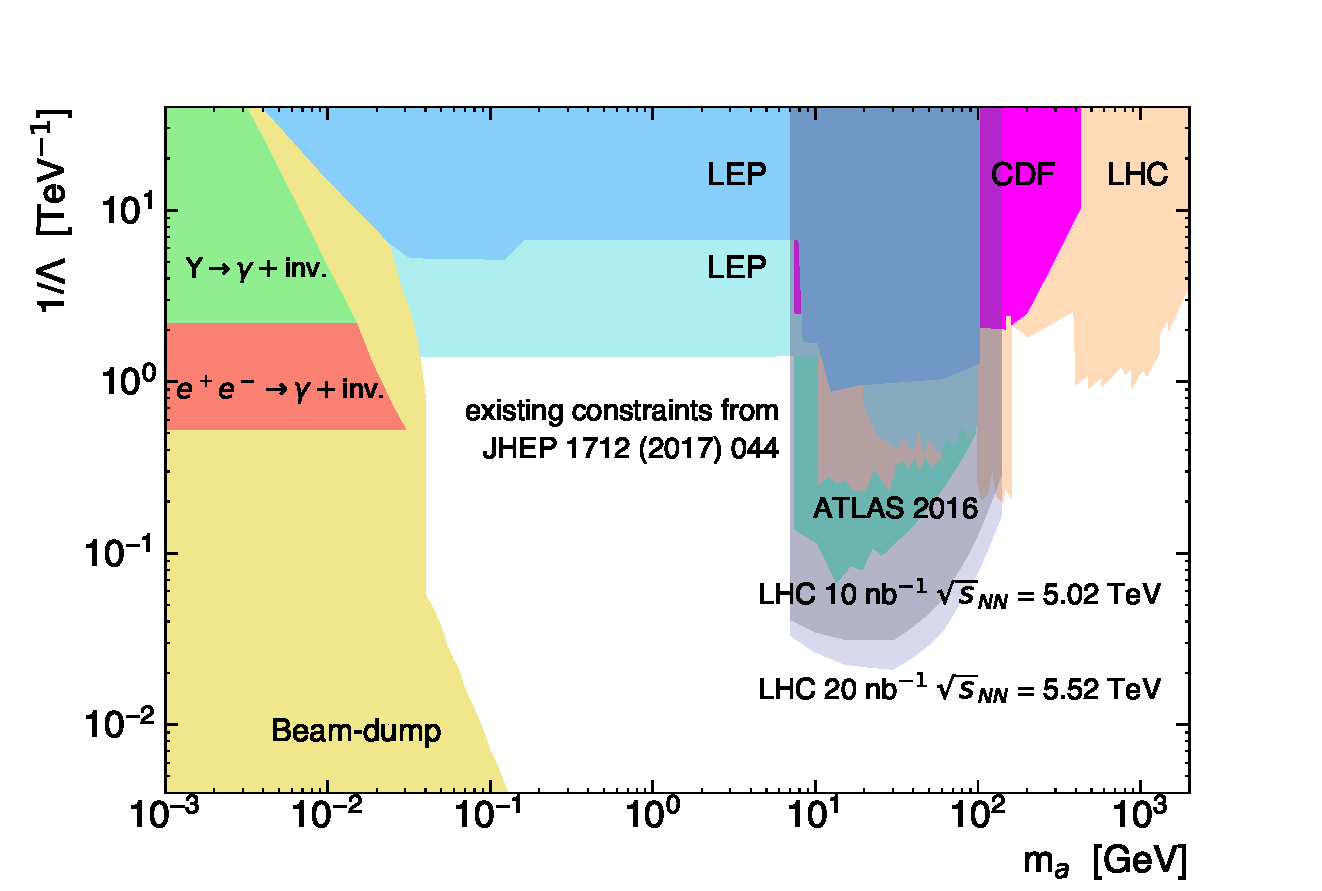
\includegraphics[scale=0.7]{\main/beyond/fig/ALPLimits_atlas_cms.pdf}
  \caption{Compilation of exclusion limits obtained by different experiments~(see text).
  ATLAS 2016 represents the exclusion limit derived from the recent LbyL cross section measured in Pb+Pb collisions by ATLAS.
  In dark grey, LHC 10~nb$^{-1}$ is shown corresponding to the analysis described in this document. Also in light grey, the LHC 20~nb$^{-1}$ limit for nominal $\sqrt{s_{\mathrm{NN}}}=5.52$~TeV is presented. A more complete version of the existing constraints on ALPs masses versus coupling, including the
  constraints in the sub meV range from astrophysical observations and
  from dedicated experiments such as CAST can be found in Ref.~\cite{Bauer:2017ris}.}
  \label{fig:alp-lambda-limits}
\end{figure}
%-------------------------------------------------------------------

%%%%%%%%%%%%%%%%%%%%%%%%%%%%%%%%%%%%%%%%%%%%%%%%%%%%%%%%%%%%%%%%%%%%%%
\subsection{Proton-oxygen collisions for cosmic ray research}
\label{sec:pOcosmic}
%%%%%%%%%%%%%%%%%%%%%%%%%%%%%%%%%%%%%%%%%%%%%%%%%%%%%%%%%%%%%%%%%%%%%%

\begin{figure}
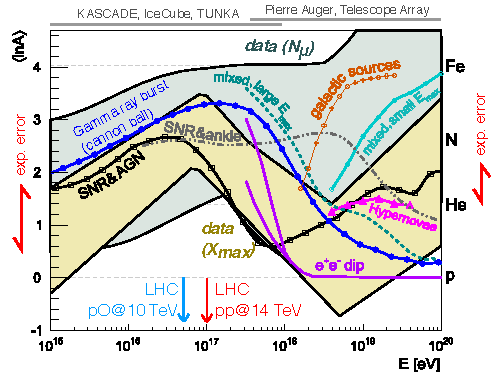
\includegraphics[width=0.5\textwidth,trim=5 -5 20 0]{\main/beyond/fig/lna_uncertainty.pdf}
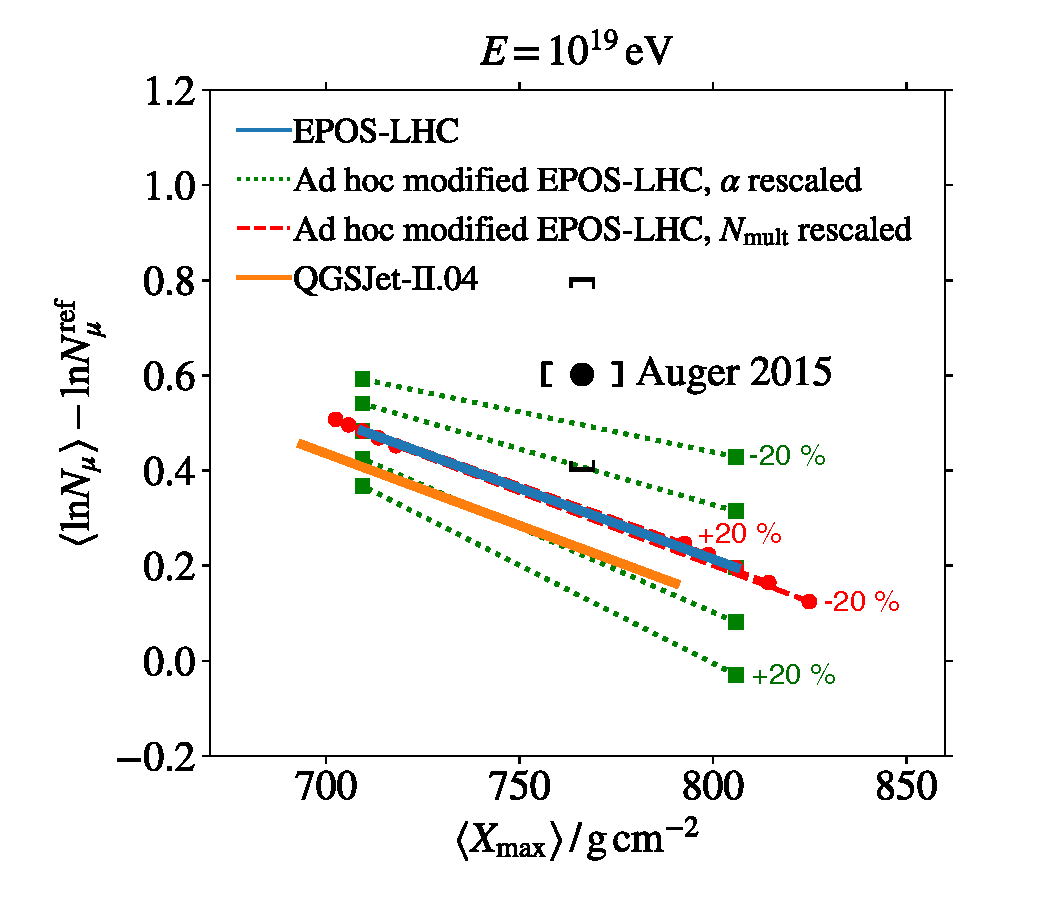
\includegraphics[width=0.5\textwidth,trim=-20 0 30 0]{\main/beyond/fig/epos_mod.pdf}
\caption{\emph{Left panel:} Mass composition of cosmic rays quantified by $\mlna$ as a function of cosmic ray energy $E$. See Ref.~\cite{kampert_cr_review} for references to data (bands) and model predictions (markers and lines), and the text for a discussion. \emph{Right panel:} Projected impact of measurements of hadron multiplicity $\nmult$ and the energy fraction $\alpha$ which goes into neutral pions in pp collisions at \SI{13}{TeV} on EPOS-LHC predictions for mean $\xmax$ and $\lnnmu$ in $10^{19}$\,\si{eV} air showers, compared to Auger data~\cite{Aab:2014pza}. The model lines represent all values that can be obtained for any mixture of cosmic nuclei from proton to iron. The dashed and dotted lines represent modifications of $\nmult$ and $\alpha$ in steps of $\pm$10\% from their nominal values.}
\label{fig:cosmic_rays}
\end{figure}

The recent coincident observations of gamma rays and neutrinos from the flaring blazar TXS 0506+056 confirmed that active galactic nuclei produce high-energy cosmic rays~\cite{IceCube:2018dnn}. This is a long awaited finding demonstrates that sources of cosmic rays are linked to the most violent places in our universe. Measurements of cosmic rays contribute to the understanding of the high-energy universe. Since cosmic rays are charged and bent onto chaotic paths by magnetic fields in space, their arrival directions are highly isotropic, but their mass composition contains a unique imprint from the source physics.

Cosmic rays are nuclei from proton to iron, with a negligible fraction of heavier elements. The mass composition of cosmic rays in a given energy interval is characteristic for different source scenarios. This is shown in Fig.~\ref{fig:cosmic_rays}, left-hand-side, where the mean-logarithmic-mass $\mlna$ of cosmic rays is shown for several source scenarios (lines and markers). The model predictions are compared to a compilation of experimental data. Above $10^{15}$\,\si{eV}, $\mlna$ can only be indirectly inferred from extensive air showers, huge secondary particle cascades produced by collisions between cosmic ray and nuclei in the atmosphere. The two leading observables to infer $\mlna$ are the depth $\xmax$ of the shower maximum in the atmosphere (yellow band in Fig.~\ref{fig:cosmic_rays}), and the number $\nmu$ of muons produced in the shower (green band in Fig.~\ref{fig:cosmic_rays}). The width of those bands has two main contributions: the experimental uncertainties, and the model uncertainties inherent in converting the air shower observables into $\mlna$.

Leading experiments achieve an experimental uncertainty of 10 to 15\% in $\mlna$ from $\xmax$ and $\nmu$, which would be sufficient to discriminate between source scenarios, but air shower simulations are required to convert $\nmu$ and $\xmax$ to $\mlna$ and this adds a large model uncertainty. The simulations use the general-purpose heavy-ion event generator EPOS-LHC~\cite{Werner:2005jf}, or more specialized hadronic interaction models such as \mbox{QGSJet-II.04}~\cite{Ostapchenko:2010vb} and SIBYLL-2.3c~\cite{Riehn:2017mfm}, which are designed to describe nucleus-nucleus and soft-QCD interactions by extrapolating using a combination of Regge field theory and perturbative QCD tuned to available data.
The uncertainties arise from a lack of data on multiparticle production in the very forward phase-space in hadron-nucleus interactions at very high energies.

Predictions for the observable $\xmax$ have converged recently thanks to LHC measurements, in particular due to high-precision measurements of the inelastic cross-section (see e.g.~\cite{Aaij:2018okq} and references therein). The predictions for $\nmu$ still vary significantly and are not consistent with $\xmax$. There is overwhelming evidence from air shower experiments~\cite{Aab:2014pza,Dembinski:2017zkb,Kokoulin:2009zz,AbuZayyad:1999xa,Aab:2014dua} that the muon number $\nmu$ is underestimated in simulations at high energies, as indicated by the data point from the Pierre Auger Observatory in Fig.~\ref{fig:cosmic_rays}, right-hand-side, which is well above the predictions from all current hadronic interaction models. This produces conflicting interpretation of the cosmic ray composition and impairs the general confidence in air shower simulations.

% The impact can be see in Fig.\ref{fig:cosmic_ray_related_lhc_measurements}, left-hand-side, which compares up-to-date models (solid lines) tuned to LHC data to predictions from older models (dashed and dotted lines).

% why we want to discuss ``forward'' in the context of ``pO''???
%The forward direction is in particular important for the air shower development, and naturally difficult to %instrument at accelerators. This results in relatively large model uncertainties due to missing constraints %by data in the relevant phase space. 

Two aspects of multi-particle production with a strong effect on $\nmu$ have been identified, the hadron multiplicity $\nmult$ and the energy fraction $\alpha$ that goes into neutral pions. The impact of changing these variables in EPOS-LHC at $13$\,TeV cms energy and extrapolating is shown in Fig.\ref{fig:cosmic_rays}, right-hand-side. A measurement to 5\,\% accuracy of both variables at the LHC would reduce the model uncertainty for the conversion of $\xmax$ to $\mlna$ below the experimental uncertainty, and has the clear potential to resolve the discrepancy in the muon number.

\begin{figure}
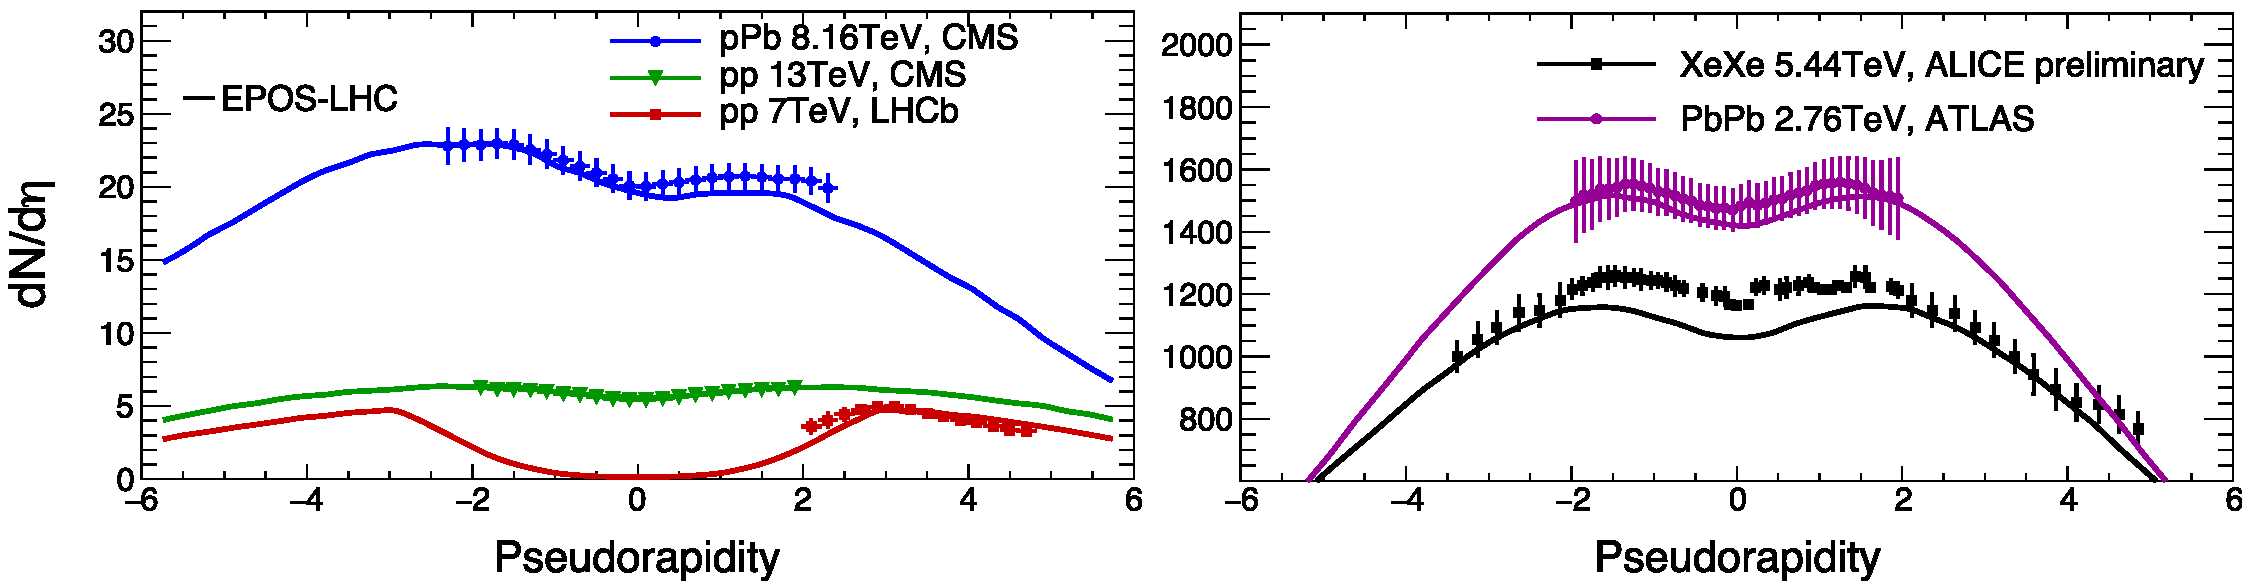
\includegraphics[width=\textwidth]{\main/beyond/fig/multiplicity_tuning_mod.pdf}
\caption{Comparison of charged particle multiplicity measurements at different center-of-mass energies and in different colliding systems with the EPOS-LHC model~\cite{Kim:2018ink}.}
\label{fig:multiplicity_tuning}
\end{figure}

Hadrons produced in the forward direction dominate the air shower development and experience significant nuclear modification\cite{Aaij:2017cqq}. The atmosphere consists of nitrogen and oxygen, therefore p-p collisions alone cannot constrain $\alpha$ and $\nmult$ to 5\,\%~\cite{dEnterria:2018kcz}. How to interpolate from p-p and p-Pb data to p-N or p-O is not clear, because the dominant nuclear effects for a light and heavy collision partner are expected to be different. Light nuclei are described by the shell model and nucleon correlations are important. Lead nuclei can be described by a simpler model, essentially a Wood-Saxon potential. The effect of correlations is reduced and cannot be probed well in experiments.
% Furthermore the collective effects which were not expected to be observed in light system (and as a consequence not implemented in specialized models for air shower simulation) seems to be very present in p-Pb~\cite{ALICE:2017jyt}.
The difficulty of predicting nuclear effects is demonstrated in Fig.~\ref{fig:multiplicity_tuning}, which shows EPOS-LHC predictions for Xe-Xe collisions, which deviate from the measurement, although EPOS-LHC provides a good description of p-p, p-Pb, and Pb-Pb data. The deviations in Xe-Xe are much larger than what is expected from a simple interpolation~\cite{Kim:2018ink}. Isolating peripheral p-Pb collisions to mimic p-O collisions with the same number of binary collisions is not a viable solution either, since this number is experimentally not well determined~\cite{Toia:2014wia}.

To achieve the desired accuracy and avoid systematic uncertainties, a direct measurement of multi-particle production of light hadrons in proton-oxygen collisions is highly desirable. The luminosity requirements to reach the physics goals are moderate. To reach a statistical accuracy of 5\,\%, 100\,M minimum-bias events are needed, which can be accumulated within a day of data-taking as described in Section~\ref{sec:pOrun}. The setup of p-O collisions would follow the successful rapid set-up procedure previously used in the 2012 p-Pb run and the 2017 Xe-Xe run.

\end{document}
